%% LyX 2.0.2 created this file.  For more info, see http://www.lyx.org/.
%% Do not edit unless you really know what you are doing.
\documentclass{UNCC-thesis}
\usepackage[T1]{fontenc}
\usepackage[latin9]{inputenc}
\setcounter{secnumdepth}{3}
\usepackage{array}
\usepackage{verbatim}
\usepackage{float}
\usepackage{graphicx}
\usepackage{nomencl}
% the following is useful when we have the old nomencl.sty package
\providecommand{\printnomenclature}{\printglossary}
\providecommand{\makenomenclature}{\makeglossary}
\makenomenclature

\makeatletter

%%%%%%%%%%%%%%%%%%%%%%%%%%%%%% LyX specific LaTeX commands.
%% Because html converters don't know tabularnewline
\providecommand{\tabularnewline}{\\}

\@ifundefined{showcaptionsetup}{}{%
 \PassOptionsToPackage{caption=false}{subfig}}
\usepackage{subfig}
\makeatother

\begin{document}
\pagenumbering{roman}
\fbmatterchapterformat
% Doctype should be either dissertation proposal, dissertation, or thesis.
% If you're getting a master's, use "thesis."  If you're getting a PhD, use "dissertation."

\doctype{thesis}


% Note: Only the first letter of the entire title should be capitalized to allow the 
% title to appear as required by the graduate school in the Abstract page.
\title{My LyX Thesis}
\author{Test User}
\degree{Master of Science}
\major{Electrical Engineering}
\publicationyear{2015}

\advisor{Dr. Person A}

% Add the full name and title of all your committee members,
% apart from your advisor, one by one.  The style file expects
% 3 to 5 committee members in addition to your advisor.

\committeeMember{Dr. Person B}
\committeeMember{Dr. Person C}


% Generate the preliminary pages (title page, copyright page, 
% abstract page, and table of contents) in the following order.
\maketitlepage

\makecopyright
\begin{abstract}
Content of your abstract goes here.\end{abstract}
\begin{acknowledgements}
Your acknowledgements go here.\end{acknowledgements}
\begin{dedication}
If you decide to have a dedication. Your dedication would go here.\end{dedication}
\begin{introduction}
If you decide to have an introduction. Your introduction would go
here. 
\end{introduction}
\tableofcontents{}

\listoffigures


\listoftables


\renewcommand{\nomname}{LIST OF ABBREVIATIONS}
% uncomment line below to title your nomenclature list as LIST OF SYMBOLS
%\renewcommand{\nomname}{LIST OF SYMBOLS}
\addcontentsline{toc}{chapter}{\nomname}\settowidth{\nomlabelwidth}{GNU}
\printnomenclature{}

\nomenclature{GNU}{GNU is not UNIX.}

\newpage
\setcounter{page}{1}
\pagenumbering{arabic}
% 2 inch top spacing for new chapters
\bodychapterformat


% Write chapter titles in ALL CAPS.


\begin{comment}
UNC Charlotte Guidelines 2014: Thesis Text (p4)

Do not use bold, underline or create unusual fonts for chapter titles;
do not use running headers or footers. Do not use bold, underline
or italics for headings, subheadings, etc. Changes in font style or
typeface are not permitted except for inclusion of illustrative or
documentary materials such as computer printouts or if required for
mathematical expressions. If you are unsure about the acceptability
of the typeface you want to use for your final copy of the thesis
or dissertation, please verify with the thesis/dissertation reviewer
in the Graduate School that it can be used.
\end{comment}



\chapter{INTRODUCTION}

This is my introduction. GNU is a major free software advocate \cite{gpl}.


\section{Problem Statement}

This is an example of a subsection.
\begin{table}[H]
\begin{centering}
{\small }%
\begin{tabular}{|c|>{\centering}p{1in}|>{\centering}p{1in}|>{\centering}p{1in}|>{\centering}p{1in}|}
\hline 
{\small Case \#} & {\small Translational displcmnt.} & {\small Total $\alpha$} & {\small Total $\beta$} & {\small Total $\gamma$ }\tabularnewline
\hline 
\hline 
{\small 6} & {\small 83.09} & {\small 885.66} & {\small 252.07} & {\small 264.64}\tabularnewline
\hline 
{\small 7} & {\small 63.12} & {\small 337.48} & {\small 244.95} & {\small 381.31}\tabularnewline
\hline 
{\small 8} & {\small 70.45} & {\small 240.08} & {\small 217.59} & {\small 294.56}\tabularnewline
\hline 
{\small 12} & {\small 15.71} & {\small 86.89} & {\small 74.58} & {\small 112.03}\tabularnewline
\hline 
\end{tabular}
\par\end{centering}{\small \par}

\caption{This is an example of a table.}
\end{table}
\begin{table}[H]
\centering{}{\small }%
\begin{tabular}{|>{\centering}p{1in}|>{\centering}p{1in}|>{\centering}p{1in}|}
\hline 
{\small R} & {\small Overall severity} & {\small KL-score}\tabularnewline
\hline 
\hline 
{\small Translation} & {\small 0.68} & {\small 0.28}\tabularnewline
\hline 
{\small{} $\alpha$} & {\small 0.34} & {\small 0.17}\tabularnewline
\hline 
{\small $\beta$} & {\small 0.59} & {\small 0.27}\tabularnewline
\hline 
{\small $\gamma$} & {\small 0.53} & {\small 0.29}\tabularnewline
\hline 
\end{tabular}\caption[Example of short label.]{This is an example of a table having a long caption whose caption
in the list of tables is much shorter (from the ``opt'' label).
Correlation coefficient (R) comparison between displacement parameters
and average overall ranking and KL score.}
\end{table}
\begin{figure}[H]
\begin{centering}
\subfloat[Translational displacement vs. Savg; a linear fit ]{\begin{centering}
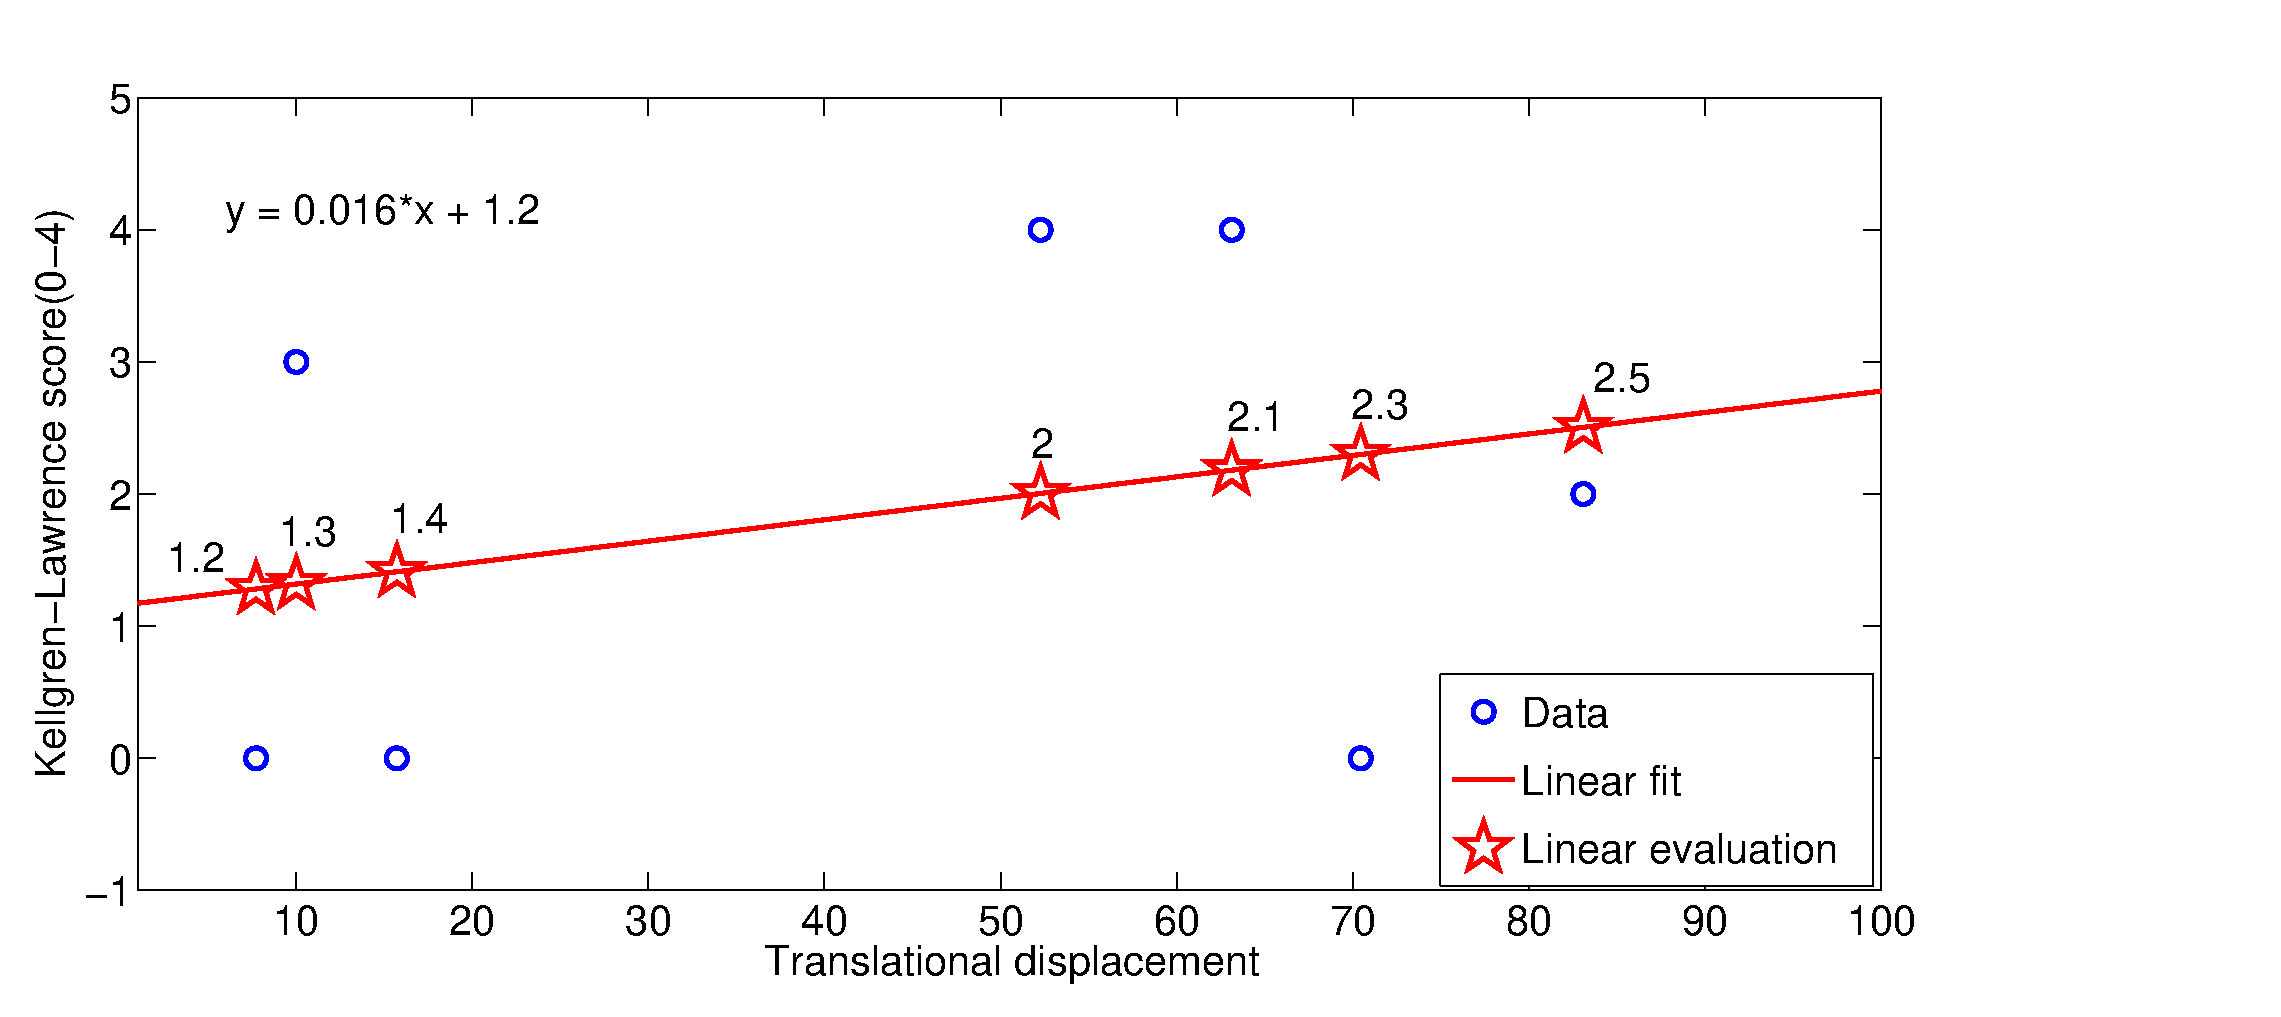
\includegraphics[height=2in]{figs/TransVsKLLine}
\par\end{centering}

}
\par\end{centering}

\begin{centering}
\subfloat[Translational displacement vs. KL; a linear fit ]{\begin{centering}
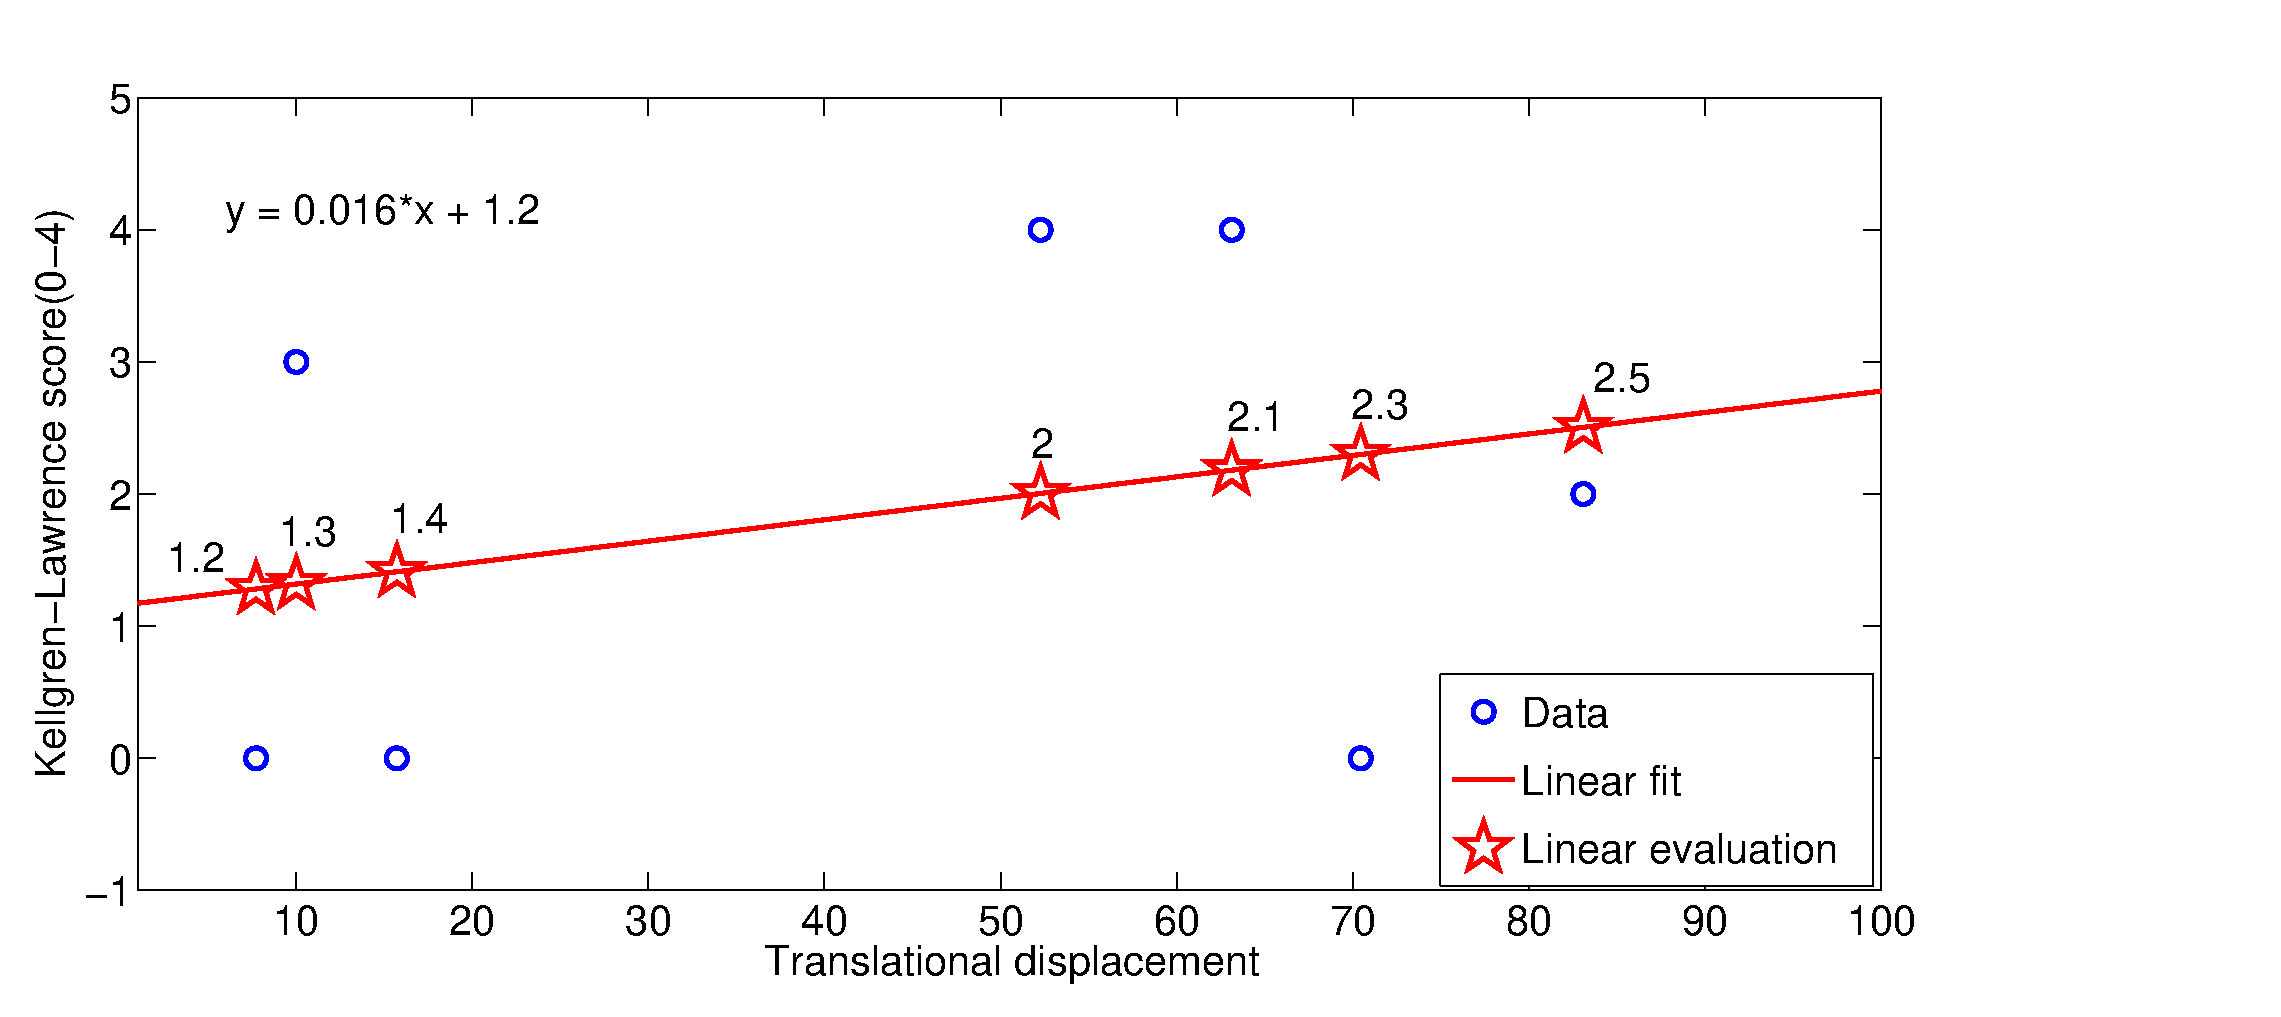
\includegraphics[height=2in]{figs/TransVsKLLine}
\par\end{centering}

}
\par\end{centering}

\caption[Shortened figure caption for list of figures.]{Linear fitting translational displacement to KL and average overall
severity.}
\end{figure}



\chapter{CONCLUSIONS}

Lots of interesting conclusions will be put here.

\fbmatterchapterformat

\bibliographystyle{plain}
\bibliography{references_db}


\newpage{}\uncctocformat{chapter}{0pt}{350pt}{\appendixname~\thecontentslabel:~}
\renewcommand{\chaptertitlename}{APPENDIX} 

\appendix

\chapter{QUADRATIC FIT COMPARISON GRAPHS}

Test of appendices.


\section{Section in appendix}

This is a section in the appendix.
\begin{vita}
If you want to include a vita, i.e., a biosketch about yourself. You
would include it here.\end{vita}

\end{document}
